\renewcommand{\arraystretch}{1.3}
%\renewcommand*{\DinoThmLogo}{\textcolor{ColorOne}{\oldpilcrowfour}\ignorespaces}
%\renewcommand*{\DinoThmLogo}{\hspace*{\DinoTitleIndent-3pt}\ignorespaces}

%\textcolor{ColorOne}{\oldpilcrowfour}\ignorespaces

%%%%%% quelques figures, le début arrive ensuite
\newcommand{\paraone}{
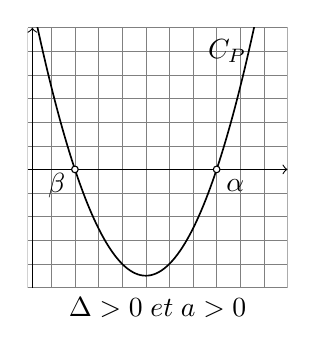
\begin{tikzpicture}[domain=-5:5,samples=100,x=6mm,y=6mm]
		\clip (-2,-3.5) rectangle (3.5,3);
	\draw[very thin,color=gray,xstep=0.5,ystep=0.5] (-2,-2.5) grid (3.5,3);
	\draw [->](-2,0) -- (3.5,0) node[above=15mm,left=4mm] {$\symcal{C}_P$};
	\draw[->] (-1.9,-2.5) -- (-1.9,3) node[above] {};
	\draw[semithick,domain=-2:3.5,label=left:$\symcal{C}_P$] plot (\x,{0.5(\x+1)*(\x-2)});
	\draw [fill=white] (-1,0) circle (1.2pt) node[below=2mm,left] {$\beta$};
\draw [fill=white] (2,0) circle (1.2pt) node[below=2mm,right] {$\alpha$};
\node[below] at (.75,-2.5){$\Delta>0\;\text{ et }\; a>0$};	
	\end{tikzpicture}
}
\newcommand{\paratwo}{	
	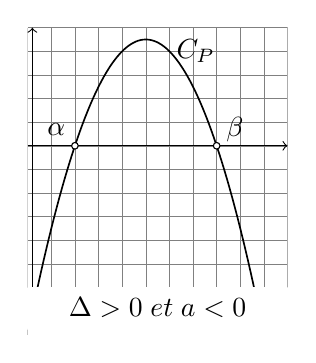
\begin{tikzpicture}[domain=-5:5,samples=100,x=6mm,y=6mm]
		\clip (-2,-4) rectangle (3.5,2.5);
	\draw[very thin,color=gray,xstep=0.5,ystep=0.5] (-2,-3) grid (3.5,2.5);
	\draw [->](-2,0) -- (3.5,0) node[above=12mm,left=8mm] {$\symcal{C}_P$};
	\draw[->] (-1.9,-3) -- (-1.9,2.5) node[above] {};
	\draw[semithick,domain=-2:3.5,label=left:$\symcal{C}_P$] plot (\x,{-(\x+1)*(\x-2)});
	\draw [fill=white] (-1,0) circle (1.2pt) node[above=2mm,left] {$\alpha$};
\draw [fill=white] (2,0) circle (1.2pt) node[above=2mm,right] {$\beta$};
\draw[fill=white,white] (-2,-4) rectangle (3.5,-3);
\node[below] at (.75,-3){$\Delta>0\;\text{ et }\; a<0$};		
	\end{tikzpicture}	
}

\newcommand{\parathree}{	
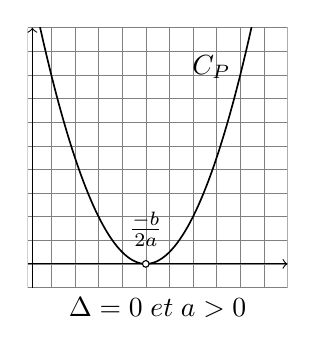
\begin{tikzpicture}[domain=-5:5,samples=100,x=6mm,y=6mm]
		\clip (-2,-1.5) rectangle (3.5,5);
	\draw[very thin,color=gray,xstep=0.5,ystep=0.5] (-2,-.5) grid (3.5,5);
	\draw [->](-2,0) -- (3.5,0) node[above=25mm,left=6mm] {$\symcal{C}_P$};
	\draw[->] (-1.9,-.5) -- (-1.9,5) node[above] {};
	\draw[semithick,domain=-2:3.5] plot (\x,{(\x+1)*(\x-2)+2.25});
	\draw [fill=white] (0.5,0) circle (1.2pt) node[above=1mm] {$\frac{-b}{2a}$};
\node[below] at (.75,-0.5){$\Delta=0\;\text{ et }\; a>0$};	
	\end{tikzpicture}
}

\newcommand{\parafour}{	
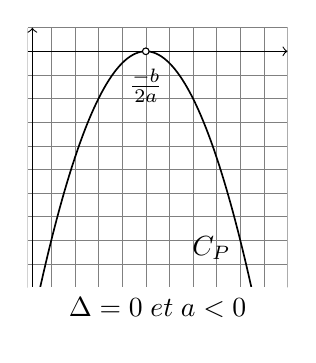
\begin{tikzpicture}[domain=-5:5,samples=100,x=6mm,y=6mm]
		\clip (-2,-6) rectangle (3.5,0.5);
	\draw[very thin,color=gray,xstep=0.5,ystep=0.5] (-2,-5) grid (3.5,.5);
	\draw [->](-2,0) -- (3.5,0) node[below=25mm,left=6mm] {$\symcal{C}_P$};
	\draw[->] (-1.9,-5) -- (-1.9,.5) node[above] {};
	\draw[semithick,domain=-2:3.5] plot (\x,{-(\x+1)*(\x-2)-2.25});
	\draw [fill=white] (0.5,0) circle (1.2pt) node[below=1mm] {$\frac{-b}{2a}$};
\draw[fill=white,white] (-2,-6) rectangle (3.5,-5);	
\node[below] at (.75,-5){$\Delta=0\;\text{ et }\; a<0$};	
	\end{tikzpicture}
}

\newcommand{\parafive}{
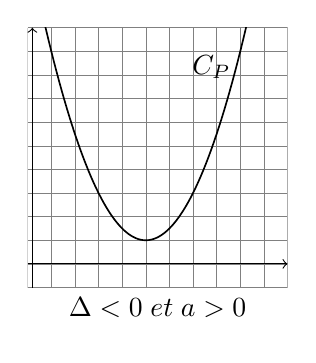
\begin{tikzpicture}[domain=-5:5,samples=100,x=6mm,y=6mm]
		\clip (-2,-1.5) rectangle (3.5,5);
	\draw[very thin,color=gray,xstep=0.5,ystep=0.5] (-2,-.5) grid (3.5,5);
	\draw [->](-2,0) -- (3.5,0) node[above=25mm,left=6mm] {$\symcal{C}_P$};
	\draw[->] (-1.9,-.5) -- (-1.9,5) node[above] {};
	\draw[semithick,domain=-2:3.5] plot (\x,{(\x+1)*(\x-2)+2.75});
\node[below] at (.75,-.5){$\Delta<0\;\text{ et }\; a>0$};		
	\end{tikzpicture}
}

\newcommand{\parasix}{	
	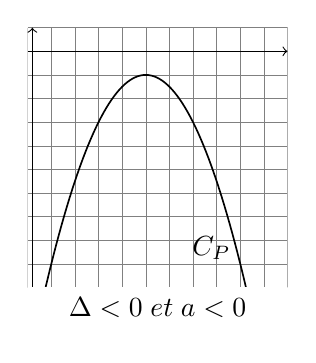
\begin{tikzpicture}[domain=-5:5,samples=100,x=6mm,y=6mm]
		\clip (-2,-6) rectangle (3.5,0.5);
	\draw[very thin,color=gray,xstep=0.5,ystep=0.5] (-2,-5) grid (3.5,.5);
	\draw [->](-2,0) -- (3.5,0) node[below=25mm,left=6mm] {$\symcal{C}_P$};
	\draw[->] (-1.9,-5) -- (-1.9,.5) node[above] {};
	\draw[semithick,domain=-2:3.5] plot (\x,{-(\x+1)*(\x-2)-2.75});
\draw[fill=white,white] (-2,-6) rectangle (3.5,-5);	
\node[below] at (.75,-5){$\Delta<0\;\text{ et }\; a<0$};	
	\end{tikzpicture}
}
%%%%
\tgotitle{Polynômes du second degré}
\tgoshorttoc
\section{Généralités}
\subsection{Fonction polynôme du second degré}
On dit qu'une fonction $P$, définie sur l'ensemble $\R$ des nombres réels et à valeurs dans $\R$, est une fonction polynôme du second degré s'il existe un réel $a$ non nul ainsi que deux réels $b$ et $c$ tels que
\[\forall x\in\R,\; P(x)=ax^2+bx+c.\]
On convient alors de dire que $ax^2+bx+c$ est un polynôme du second degré.

\begin{remark}
Cette définition n'entraîne évidemment pas qu'une fonction polynôme de degré 2 donnée ne puisse pas s'écrire sous une forme différente. Par exemple :
\begin{itemize}
\item Cas de $P : \R\rightarrow\R,\; x\mapsto x^2-3x+2$ : $\forall\,x\in\R$, $P(x)=(x-1)(x-2)$.
\item  Cas de $Q : \R\rightarrow\R,\; x\mapsto x^2-1$ : $\forall\,x\in\R$,
 \[Q(x)=\frac{x^4-1}{x^2+1}.\]
 \item Cas de $R : \R\rightarrow\R,\; x\mapsto x^2-2x+5$ : $\forall\,x\in\R$, $R(x)=\left(\left({x-1}\right)^2\right)+4$.
\end{itemize}
\end{remark}
\subsection{Écriture unique}
Il existe cependant un certaine unicité de l'écriture d'un polynôme de degré~2, qui concerne plus précisément ses \emph{coefficients} $a$, $b$ et $c$.
\begin{thm}
Soit $(a,a')\in\R^*\times\R^*$, $(b,b')\in\R\times\R$ et $(c,c')\in\R\times\R$ tels que
\[\forall x\in\R,\; ax^2+bx+c=a'x^2+b'x+c',\]
alors $a=a'$, $b=b'$ et $c=c'$. 
\label{thunicite}
\end{thm}
\begin{proof}
L'égalité entre les deux expressions étant vraie pour tout $x\in\R$, elle l'est en particulier pour $x=0$. On en déduit que $c=c'$ et par conséquent
\begin{align*}
\forall x\in\R,\; ax^2+bx&=a'x^2+b'x,\\
\forall x\in\R,\; x(ax+b)&=x(a'x+b'),\\
\intertext{Soit, en simplifiant par $x\neq0$}
\forall x\in\R^*,\;ax+b&=a'x+b'.
\end{align*}

En donnant alors successivement à $x$ les valeurs $1$ et $2$, on obtient :
\[\left\{\begin{aligned}
(a-a')+(b-b')&=0\\
2(a-a')+(b-b')&=0
\end{aligned}\right.\;,\]
dont la résolution amène à $a-a'=0$ et $b-b'=0$, c.-à-d. : $a=a'$ et $b=b'$.
\end{proof}

\section{Forme canonique}
\subsection{Méthode de complétion au carré}\label{sec2-1}
Fixons nous un réel $m$. On rappelle que, pour tout $x\in\R$, $(x+m)^2=x^2+2mx+m^2$. Ou encore :
\begin{equation}
\forall x\in\R, \; x^2+2mx=\left(x+m\right)^2-m^2.
\end{equation}

Dans le cas de $P : \R\rightarrow\R, x\mapsto x^2+2mx+p$, on remarque que l'on peut alors écrire 
\begin{equation}
x^2+2mx+p=\left(x+m\right)^2-m^2+p.\label{eqfcreduite}
\end{equation}

Cette remarque fonde la \emph{méthode de complétion au carré}.

\begin{example}[Exemples]
\begin{enumerate}
\item  \label{explefactor} 
On souhaite résoudre l'équation $x^2-6x+7=0$. On remarque que \[x^2-6x+7=(x-3)^2-9+7\] et on se ramène ainsi à
\begin{align*}
(x-3)^2-2&=0,\\
(x-3)^2-\bigl(\sqrt{2}\bigr)^2&=0,\\
\intertext{puis en employant une identité remarquable}
\bigl(x-3+\sqrt{2}\bigr)\bigl(x-3-\sqrt{2}\bigr)&=0.
\end{align*}
D'où l'on déduit que l'ensemble des solutions de $x^2-6x+7=0$ est 
\[
\symcal{S}=\bigl\{3-\sqrt{2}, 3+\sqrt{2}\bigr\}.
\]
\item Démontrer que $x^2+x+1$ est strictement positif pour tout $x\in\R$.
On écrit 
\begin{align*}
x^2+x+1&=x^2+2\times\frac12x+1,\\
&=\left(x+\frac12\right)^2-\frac14+1,\\
&=\left(x+\frac12\right)^2+\frac34\,.
\end{align*}

On en déduit que, pour tout $x\in\R$,
\[x^2+x+1≥\frac34\:.\]
On a donc finalement : $\forall x\in\R,\; x^2+x+1>0$.
\end{enumerate}
\end{example}
\subsection{Cas général}
En factorisant $a$ dans  $P(x)$, on obtient le théorème suivant :
\begin{thm}
Soit $P$, la fonction polynôme de degré 2 définie sur $\R$ par $P(x)=ax^2+bx+c$. On a 
\begin{equation}
\forall x\in\R,\;P(x)=a\left(\left(x+\frac{b}{2a}\right)^2-\frac{\Delta}{4a^2}\vphantom{\frac{b^2}{4a^2}}\right),\label{eqformcan}
\end{equation}
où $\Delta$, que l'on nomme \emph{discriminant} du polynôme $P(x)$, vaut $\Delta=b^2-4ac$.
\label{thformcan}
\end{thm}
\begin{proof}
On commence par factoriser $a$ dans $P(x)$ :
\[P(x)=a\left(x^2+\frac{b}{a}x+\frac{c}{a}\right),\]
puis on utilise l'égalité \eqref{eqfcreduite} avec $m=b/(2a)$ et $p=c/a$. On obtient 
\[P(x)=a\left(\left(x+\frac{b}{2a}\right)^2-\frac{b^2}{4a^2}+\frac{c}{a}\right).
\]
%D'où le résultat annoncé.
Une réduction au même dénominateur amène alors au résultat annoncé.
\end{proof}

\subsubsection{Discriminant réduit}
Dans le cas où $b$ se met agréablement sous la forme $2b'$ (par exemple, lorsque $b$ est un entier pair) on peut remarquer que $b/2a=b'/a$ et que $\Delta=4b'^2-4ac$.
 On est alors amené à poser $\Delta'=b'^2-ac$ et l'on obtient
\begin{equation}
\forall x\in\R,\;P(x)=a\left(\left(x+\frac{b'}{a}\right)^2-\frac{\Delta'}{a^2}\vphantom{\frac{b^2}{4a^2}}\right).
\end{equation}
Le nombre $\Delta'$ est souvent nommé \emph{discriminant réduit}

\subsubsection{Extrémums}
La forme canonique de la fonction $P$ met en évidence l'existence d'un extrémum dont la nature dépend du signe de $a$.
\begin{thm}
Soit $P$, la fonction polynôme de degré 2 définie sur $\R$ par $P(x)=ax^2+bx+c$. 
\XSmartphoneCommand{\vspace{\baselineskip}}

La fonction $P$ admet en\SmartphoneCommand{\\} $-\dfrac{b}{2a}\left\{\begin{aligned} 
\text{un \emph{minimum} égal à $\smash{-\dfrac{\Delta}{4a}}$}\; &\text{si $a>0$,}\\[2.5ex]
\text{un \emph{maximum} égal à $\smash{-\dfrac{\Delta}{4a}}$}\; &\text{si $a<0$.}
\end{aligned}\right.$
\vspace{1ex}\par
\label{thextrem}
\end{thm}

\begin{proof}
On voit tout d'abord que 
\[\forall x\in\R,\;\left(x+\frac{b}{2a}\right)^2≥0,
\]
donc que
\[
\forall x\in\R,\;\left(x+\frac{b}{2a}\right)^2-\frac{\Delta}{4a^2}≥-\frac{\Delta}{4a^2},
\]
l'égalité n'étant atteinte que si le carré est nul, donc si $x=-b/(2a)$. On fait alors apparaître $P(x)$ (compte tenu de l'égalité \eqref{eqformcan} du théorème \ref{thformcan}) en multipliant chaque membre de cette inégalité par $a\neq0$, ce qui change ou non son sens, selon que a est positif ou négatif. Il vient alors :
\begin{itemize}
\item si $a>0$, 
\[
\forall x\in\R,\; P(x)≥-\frac{\Delta}{4a}\;;
\]
\item et si $a<0$, 
\[
\forall x\in\R,\; P(x)≤-\frac{\Delta}{4a}\,.
\]
\end{itemize}
On sait de plus que dans les deux cas, l'égalité est atteinte si et seulement si $x=-b/(2a)$.
\end{proof}

\section{Factorisation}
\subsection{Théorème de factorisation}
La méthode vue dans l'exemple \ref{explefactor} de la section \ref{sec2-1} se généralise, pourvu que $\Delta$ soit positif. Précisément, on a le théorème 
\begin{thm}\label{thfactor}%
Soit $P$, la fonction polynôme de degré 2 définie sur $\R$ par $P(x)=ax^2+bx+c$.  Si le discriminant $\Delta$ de $P$ est positif ($\Delta≥0$), alors
\begin{align*}
\forall x \in\R,\;P(x)&=a(x-\alpha)(x-\beta)\\
\text{où}\quad\alpha=\frac{-b+\sqrt{\Delta}}{2a}&\text{ et }\beta=\frac{-b-\sqrt{\Delta}}{2a}.
\end{align*}
\end{thm} 
\begin{remark}
Le cas où $\Delta=0$ est particulier, puisque l'on a alors 
\[
\alpha=\beta=\frac{-b}{2a}\quad\text{soit :}\quad\forall x\in\R,\;P(x)=a\left(x-\frac{-b}{2a}\right)^2.
\]
\end{remark}

\begin{proof}
On remarque que si $\Delta≥0$, on peut écrire
\[
\frac{\Delta}{4a^2}=\left(\frac{\sqrt{\Delta}}{2a}\right)^2.
\] 

En reportant dans l'égalité \eqref{eqformcan} du théorème \ref{thformcan}, on obtient
\[
\forall x\in\R,\;P(x)=a\left(\left(x+\frac{b}{2a}\right)^2-\left(\frac{\sqrt{\Delta}}{2a}\right)^2\right).
\]

On obtient alors le résultat annoncé en factorisant la différence de deux carrés grâce à l'identité remarquable $A^2-B^2=(A+B)(A-B)$.
\end{proof}

\subsection{Racines}
Soit $P$ une fonction polynôme du second degré. 
On dit que $P$ est factorisable par $(x-x_0)$ s'il existe $m\in\R^*$ et $p\in\R$ tels que
\begin{equation}\forall x\in\R,\;P(x)=(x-x_0)(mx+p).\label{eqfactorx0}\end{equation}
On dit qu'un réel $x_0$ est une racine de $P$ si $P(x_0)=0$ : une racine de $P$ n'est donc rien d'autre qu'une solution de l'équation $P(x)=0$.

Nous pouvons maintenant formuler le théorème qui suit :
\begin{thm}
Soit $P$ une fonction polynôme du second degré et $x_0\in\R$. Le réel $x_0$ est une racine de $P$ si et seulement si $P$ est factorisable par $(x-x_0)$.
\end{thm}

\begin{proof}
Tout d'abord, si $P$ est factorisable par $x_0$, il suffit de calculer $P(x_0)$ en utilisant l'égalité \eqref{eqfactorx0} pour constater que $P(x_0)=0$, donc que $x_0$ est une racine de $P$.

Réciproquement supposons que $x_0$ est une racine de $P$, donc que $P(x_0)=0$. Soit alors $a$, $b$ et $c$ les coefficients de $P(x)$ : on a 
\[ax_0^2+bx_0+c=P(x_0)=0,\]
 d'où $c=-ax_0^2-bx_0$. Et en substituant cette écriture de $c$ dans l'expression de $P(x)$ :
\begin{align*}
P(x)&=ax^2+bx+c\\
&= ax^2+bx-ax_0^2-bx_0,\\
&= a(x^2-x_0^2)+b(x-x_0),\\
&= a(x-x_0)(x+x_0)+b(x-x_0),\\
&=(x-x_0)(ax+ax_0+b).
\end{align*}

On en arrive à $P(x)=(x-x_0)(mx+p)$, en prenant $m=a$ et $p=ax_0+b$.
\end{proof}

\subsubsection{Racines et équation du second degré}
Nous faisons ici le point sur les racines de $P$, autrement dit sur la résolution de l'équation 
$P(x)=0$.


\begin{itemize}
\item  \textit{Si $\Delta<0$,} nous reprenons le théorème \ref{thextrem} : dans ce cas, la fonction $P$ possède un minimum strictement positif si $a>0$ ou un maximum strictement négatif si $a<0$. Dans chaque cas, si $\Delta<0$, l'équation $P(x)=0$ ne possède pas de solution, autrement dit $P$ n'admet aucune racine.

\item  \textit{Si maintenant $\Delta=0$,} la remarque qui suit le théorème \ref{thfactor} prouve que l'équation $P(x)=0$ équivaut à
\[
\left(x-\frac{-b}{2a}\right)^2=0
\]
 et admet $-b/(2a)$ pour seule solution, ou encore que ce nombre est la seule racine de $P$. Dans la mesure où le facteur $x-(-b/(2a))$ intervient par son carré, on parle alors de \emph{racine double}.
 
 \item  \textit{Enfin si $\Delta>0$,} d'après le théorème \ref{thfactor}, $P(x)=0$ équivaut à $(x-\alpha)(x-\beta)=0$.
%\DinoXiPadminiCommand{$(x-\alpha)(x-\beta)=0$.}
%\DinoiPadminiCommand{\[(x-\alpha)(x-\beta)=0.\]}
 Cette équation admet donc deux solutions, ou encore $P$ admet deux racines qui sont
 \[
 \alpha=\frac{-b+\sqrt{\Delta}}{2a}\quad\text{et}\quad\beta=\frac{-b-\sqrt{\Delta}}{2a}.
 \]
\end{itemize}


\begin{remark}
Dons le cas où l'on a posé $b=2b'$ et utilisé le discriminant réduit $\Delta'$, il est facile de vérifier que les racines s'expriment comme suit :
\[
\alpha=\frac{-b'+\sqrt{\Delta'}}{a}\quad\text{et}\quad\beta=\frac{-b'-\sqrt{\Delta'}}{a}.
\]
\end{remark}

\begin{example}[Exemples]
\begin{enumerate}
\item Résoudre l'équation $3x^2-5x+1=0$ : calculons $\Delta=25-12=13$. L'équation a deux solutions qui sont les racines de $3x^2-5x+1$ :
\[
\alpha=\frac{5+\sqrt{13}}{6}\quad\text{et}\quad\beta=\frac{5-\sqrt{13}}{6}.
\]
L'ensemble des solutions est $\symcal{S}=\{\alpha,\beta\}$.
\item Factoriser si possible $-2x^2+3x+2$ : on calcule $\Delta=9+16=5^2$. Il existe deux racines qui sont $2$ et $-1/2$ ; d'où
\[
\forall x\in\R,\;-2x^2+3x+2=-2(x-2)\left(x+\frac12\right).
\]
\item Factoriser si possible $A(x)=2x^2-8$ : utilisons  l'identité remarquable 
\[
a^2-b^2=(a+b)(a-b).
\]
\[\forall x\in\R,\;2x^2-8=2(x^2-4)=2(x-2)(x+2).\]
Dans un cas de ce genre, il est bien sûr inutile de calculer $\Delta$. En revanche, l'existence de deux racines distinctes nous prouve que $\Delta>0$.
\item Résoudre l'équation $3x^2+2=0$. La fonction polynôme $x\mapsto3x^2+2$ admet un minimum strictement positif égal à $2$. Il n'y a aucune solution, l'ensemble des solutions est $\symcal{S}=\emptyset$.
\item Factoriser $9x^2-6x+1=0$. On pourrait envisager de calculer $\Delta$, mais en observant l'expression, on reconnait un membre d'identité remarquable :
\[\forall x\in\R,\;9x^2-6x+1=(3x-1)^2.\]
\item Résoudre $x^2+2x=0$. La factorisation est immédiate :
\[x^2+2x=0\iff x(x+2)=0\iff x=0\text{ ou }x+2=0.\]
L'ensemble des solutions de cette équation est donc $\symcal{S}=\{0,-2\}$.
\end{enumerate}
\end{example}
%
%

\subsection{Problème de signe}
Nous rappelons ici que la fonction \emph{signe} est définie sur $\R$ comme suit :
\[\forall x \in \R,\; \sgn(x)=\begin{cases}
-1 &\text{si $x<0$,}\\
0 &\text{si $x=0$,}\\
1 &\text{si $x>0$.}
\end{cases}
\]
Cette définition est beaucoup plus pertinente que l'usage des symboles ${+}$ et ${-}$, ne serait-ce que parce qu'elle rend exacte et claire une formulation comme \emph{le signe du produit est le produit des signes}.
\begin{thm}
Soit $P$, la fonction polynôme de degré 2 définie sur $\R$ par $P(x)=ax^2+bx+c$. 
\begin{itemize}
\item  Si $\Delta<0$,  le signe de $P(x)$ est égal à celui de $a$ en tout $x$ réel.
\item  Si $\Delta=0$, le signe de $P(x)$ est égal au signe de $a$ en tout $x$ réel différent de $-b/(2a)$ et s'annule en $-b/(2a)$.
\item  Si $\Delta>0$, le signe de $P(x)$ est égal au signe de $-a$ en tout $x$ intérieur à l'intervalle des racines, au signe de $a$ en tout $x$ extérieur à l'intervalle des racines et s'annule aux racines. 
\end{itemize}
\label{thsgn}
\end{thm}

Ces résultats s'interprètent sur la représentation graphique $\symcal{C}_P$ de $P$, selon les signes de $\Delta$ et $a$ (voir figure \ref{figracines}).
\afterpage{\clearpage\begin{figure}[H]\centering
\AfourCommand{%
\noindent\hfill\paraone\hfill\parathree\hfill\parafive\hfill\null
\par
\noindent\hfill\paratwo\hfill\parafour\hfill\parasix\hfill\null
}
\BigTabletCommand{%
\noindent\hfill\paraone\hfill\parathree\hfill\parafive\hfill\null
\par
\noindent\hfill\paratwo\hfill\parafour\hfill\parasix\hfill\null
}
\TabletCommand{%
\noindent\hfill\paraone\hfill\parathree\hfill\parafive\hfill\null
\par
\noindent\hfill\paratwo\hfill\parafour\hfill\parasix\hfill\null
}
\SmartphoneCommand{%
\noindent\hfill\paraone\hfill\paratwo\hfill\null
\par
\noindent\hfill\parathree\hfill\parafour\hfill\null
\par
\noindent\hfill\parafive\hfill\parasix\hfill\null
}
\SmallTabletCommand{%
\vspace*{1.5cm}\par
\noindent\hfill\paraone\hfill\paratwo\hfill\null
\par
\noindent\hfill\parathree\hfill\parafour\hfill\null
\par
\noindent\hfill\parafive\hfill\parasix\hfill\null
}
\figcaption{}\label{figracines}
\end{figure}
}

\begin{proof}
Examinons successivement les trois cas du théorème.
\begin{itemize}
\item  Si $\Delta<0$, le résultat provient d'une remarque déjà faite : dans ce cas, la fonction $P$ possède un minimum strictement positif si $a>0$ ou un maximum strictement négatif si $a<0$. 
\item  Si $\Delta=0$, on a 
\[
P(x)=a\left(x+\frac{b}{2a}\right)^2.
\]
% La fonction $P$ admet donc $0$ pour minimum lorsque $a>0$ ou pour maximum lorsque $a>0$. Dans les deux cas cet extrémum n'est atteint qu'une fois en $-b/(2a)$.
Le résultat annoncé se déduit du tableau de signes
\[\begin{array}{c|ccccc}
\hline
x&-\infty&&-b/(2a)&&\infty\\
\hline
\sgn\bigl(\bigl(x+\frac{b}{2a}\bigr)^2\bigr)&&1&0&1&\\
\hline
\sgn(P(x))&&\sgn(a)&0&\sgn(a)&\\
\hline
\end{array}\]
\item  Si $\Delta>0$, on constate, en se référant à l'expression des racines $\alpha$ et $\beta$ dans théorème \ref{thfactor}, que $\alpha$ est la plus grande des deux racines si $a>0$ et la plus petite si $a<0$. En posant
\begin{align*}\alpha'=\min(\alpha,\beta)&\text{ et }\beta'=\max(\alpha,\beta),\\
\intertext{on obtient}
P(x)=a(x-\alpha')(x-\beta'),\quad&\text{ avec $\alpha'<\beta'$}.
\end{align*}
On établit alors le tableau de signes
{\SmartphoneCommand{\small}
\[\begin{array}{c|ccccccc}
\hline
x&-\infty&&\alpha'&&\beta'&&\infty\\
\hline
\sgn(x-\alpha')&&-1&0&1&1&1&\\
\hline
\sgn(x-\beta')&&-1&-1&-1&0&1&\\
\hline
\sgn(P(x))&&\sgn(a)&0&\sgn(-a)&0&\sgn(a)&\\
\hline
\end{array}
\]}
Le résultat annoncé s'en déduit.\qedhere
\end{itemize}
\end{proof}

\begin{example}[Exemples]
\begin{enumerate}
\item Résoudre $x^2-x-6≤0$ : le discriminant vaut $\Delta=1+24=25$. Il existe deux racines qui sont $-2$ et $3$. On veut que $x^2-x-6$ soit négatif donc nul ou du signe de~$-a$ : cela se produit aux racines ou à l'intérieur de l'intervalle des racines. L'ensemble des solutions est $\symcal{S}=[-2,3]$.

On aurait pu également, une fois les racines calculées, utiliser la forme factorisée du polynôme $P(x)=x^2-x-6$. Ainsi $P(x)=(x+2)(x-3)$, d'où le tableau de signes :
\[\begin{array}{c|ccccccc}
\hline
x&-\infty&&\quad-2\quad&&\quad3\quad&&\infty\\
\hline
\sgn(x+2)&&-1&0&1&1&1&\\
\hline
\sgn(x-3)&&-1&-1&-1&0&1&\\
\hline
\sgn(P(x))&&1&0&-1&0&1&\\
\hline
\end{array}
\]
On retrouve la solution donnée par la première méthode.

\item Résoudre $(2x-6)^2>0$ : ce carré est positif pour tout $x\in\R$ et s'annule si et seulement si $x=3$. Par conséquent, l'ensemble des solutions de cette inéquation est $\symcal{S}=\R\smallsetminus\{3\}$. Si l'on avait eu la très mauvaise idée de développer pour calculer le discriminant, on aurait trouvé $\Delta=0$ et une racine double égale à $3$.
\item Résoudre $3x^2-4x-1≥0$ : c'est l'occasion d'utiliser le discriminant réduit.

On trouve $\Delta'=4+3=7$.
Il existe deux racines :
\[
\alpha=\frac{2+\sqrt{7}}{3}\quad\text{et}\quad\beta=\frac{2-\sqrt{7}}{3}.
\]
On veut que $3x^2-4x-1$ soit positif, donc nul ou du signe de $a$ : cela se produit aux racines ou à l'extérieur de l'intervalle des racines. L'ensemble des solutions est donc
\[
\symcal{S}=\left]-\infty, \beta\right] \cup \left[\alpha, \infty\right[.
\]
\item Résoudre $5x-2x^2>0$. La factorisation se fait à vue : 
\[
5x-2x^2=-2x\left(x-\frac52\right),
\]
 il y a donc deux racines : $\alpha=0$ et $\beta=5/2$.

On peut ensuite soit faire un tableau de signes, soit utiliser le théorème \ref{thsgn}, ce que nous ferons ici.
On veut que $5x-2x^2$ soit strictement positif,  donc du signe de $-a$ : cela se produit si et seulement si $x$ est à l'intérieur de l'intervalle des racines. L'ensemble des solutions est donc 
$\symcal{S}=\left]0,\, 5/2\right[$.
\item Résoudre $x^2-x+1>0$ : on trouve $\Delta=-3$. Il n'y a pas de racines, donc $x^2-x+1$ admet pour signe $1$ pour tout $x\in\R$. Tout $x$ réel est donc solution : l'ensemble des solutions est $\symcal{S}=\R$. 
\end{enumerate}
\end{example}
\section{Somme et produit des racines}
\subsection{Expression de la somme et du produit des racines}
On suppose ici que $\Delta≥0$, c'est-à-dire que le polynôme $P$ deux racines $\alpha$ et $\beta$, confondues en une racine double au cas où $\Delta=0$. On a le théorème suivant:
\begin{thm}\label{thsomprod}%
Soit $P$, la fonction polynôme de degré 2 définie sur $\R$ par $P(x)=ax^2+bx+c$. Si le discriminant $\Delta$ de $P$ est positif, la somme et le produit  des racines de $P$ sont données par
\[
\alpha+\beta=-\frac{b}{a} \quad\text{et}\quad \alpha\beta=\frac{c}{a}\:.
\]
\end{thm}

\begin{remark}
On sait que si $\Delta=0$, on a $\alpha=\beta=-b/(2a)$. On retrouve bien 
\[\alpha+\beta=2\times\left(-\frac{b}{2a}\right)=-\frac{b}{a}\;;\]
on remarque également que, puisque $\Delta=0$, on a $b^2=4ac$ et par conséquent
\[
\alpha\beta=\left(-\frac{b}{2a}\right)^2=\frac{b^2}{4a^2}=\frac{4ac}{4a^2}=\frac{c}{a}\:.
\]
\end{remark}

\begin{proof}On utilise  la forme factorisée de $P(x)$ :
\begin{align*}
\forall x\in\R,\;P(x)&=a(x-\alpha)(x-\beta),\\
&=a(x^2-\alpha x-\beta x +\alpha\beta),\\
&=a\left(x^2-(\alpha+\beta)x+\alpha\beta\right),\\
&=ax^2-a(\alpha+\beta)x +a\alpha\beta.
\end{align*}

D'après le théorème \ref{thunicite}, on peut identifier les coefficients : $-a(\alpha+\beta)=b$ et $a\alpha\beta=c$. Le résultat annoncé en découle immédiatement.
\end{proof}
\subsubsection{Racine apparente ou connue}
On dit que $\alpha$ est une \frquote{racine apparente} (on dit également \frquote{évidente}) du polynôme $P$ lorsqu'un simple calcul à vue permet de montrer que $P(\alpha)=0$. On parle de racine connue lorsqu'un calcul antérieur a permis d'établir cette égalité. Dans une telle situation, il est facile de déterminer $\beta$, l'autre racine de $P$, grâce à la somme ou au produit :
\[
 \beta=-\frac{b}{a}-\alpha \quad \text{ou (dans le cas où $\alpha\neq0$)}\quad\beta=\frac{c}{a\alpha}.
\]
\begin{example}[Exemples]
\begin{enumerate}
\item Factoriser le polynôme $P$, défini sur $\R$ par $P(x)=3x^2+9x+6$. Un calcul immédiat montre que $P(-1)=0$ : le réel $-1$ est donc racine de $P$, tandis que l'autre racine $\beta$ vérifie~\mbox{$-1\times\beta=6/3=2$}. D'où $\beta=-2$ et la factorisation : \[P(x)=3(x+1)(x+2).\]
\item On pose $Q(x)=2x^2-13x+15$. Calculer $Q(5)$ et résoudre l'équation $Q(x)=0$. On trouve $Q(5)=0$ : le réel $5$ est donc racine de $Q$. L'autre racine vérifie $5+\beta=6{,}5$, d'où $\beta=1{,}5$ : l'ensemble des solutions de l'équation proposée est \[\symcal{S}=\left\{5, \frac32\right\}\,.\]

\end{enumerate}
\end{example}

\subsection{Trouver deux nombres connaissant leur somme et leur produit}

\begin{thm}
Deux réels $s$ et $p$ étant donnés, il existe deux nombres réels $\alpha$ et $\beta$ dont la somme vaut $s$ et le produit $p$ si et seulement si le nombre $\Delta=s^2-4p$ est positif. Dans ce cas, les  nombres $\alpha$ et $\beta$ sont les racines de la fonction polynôme de degré $2$ définie par  $P(x)=x^2-sx+p$, de discriminant $\Delta$.
\end{thm}
\begin{proof}
\begin{itemize}
\item Tout d'abord, si $s^2-4p≥0$, la fonction  polynôme $P$, de discriminant $\Delta=s^2-4p$ admet deux racines dont la somme est $s$ et le produit $p$ d'après le théorème \ref{thsomprod}.

\item Réciproquement, s'il existe deux nombres $\alpha$ et $\beta$ tels que 
\[ 
\alpha+\beta=s \quad\text{et}\quad \alpha\beta=p,
\]
on a, d'après la première équation, $\beta=s-\alpha$, puis en substituant dans la seconde 
\[\alpha(s-\alpha)=p\quad\text{soit}\quad\alpha^2-s\alpha+p=0,\]
c'est-à-dire $P(\alpha)=0$.

Il est donc nécessaire que $\alpha$ soit une racine de $P$, ce qui entraîne que le discriminant $s^2-4p$ soit positif. Enfin, la relation $\beta=s-\alpha$ entraîne que $\beta$ est alors la seconde racine de $P$.\qedhere
\end{itemize}
\end{proof}
\begin{example}[Exemples]
\begin{enumerate}
\item Trouver deux nombres dont la somme vaut $1$ et le produit $-12$. Ces deux nombres doivent être racines de $x^2+x-12$ dont le discriminant est $49$ et qui admet $-3$ et $4$ pour racines. Les deux nombres cherchés sont donc $-3$ et $4$.
\item Trouver deux nombres dont la somme vaut $6$ et le produit $9$. On forme le polynôme $x^2-6x+9$, égal à $(x-3)^2$, dont le discriminant est nul et qui admet $3$ pour racine double : les nombres $\alpha$ et $\beta$ dont le produit vaut $9$ et la somme $6$ sont tous deux égaux à $3$.
\item Trouver deux nombres dont la somme vaut $s=5$ et le produit $p=8$. On calcule $s^2-4p=-7$ : le problème n'a pas de solution (tout comme le polynôme $x^2-5x+8$ n'admet pas de racines). 
\end{enumerate}
\end{example}
\endinput

